\documentclass{article}
\usepackage[margin=1.0in]{geometry}
% -----PACKAGES
%\usepackage[shortend,titlenumbered]{algorithm2e}
%\usepackage{algorithmic}
%\usepackage[plain]{algorithm}
\usepackage{multicol}
\usepackage{color}
\usepackage{multirow}
\usepackage{fancybox}
%\usepackage{index}
\usepackage{varioref}
\usepackage{psfrag}
\usepackage{epsfig}
\usepackage{boxedminipage}
\usepackage{graphicx}
\usepackage{rotating}
\usepackage{amsmath}
\usepackage{amssymb}
%\usepackage{amsfont}
\usepackage{latexsym}
\usepackage{alltt}
%\usepackage[small,bf]{caption}
\usepackage{url}
%\usepackage{citesort}
%\usepackage{crop}
\usepackage{array}
\usepackage{subfigure}
\usepackage{dcolumn}

% -----SETLENGTH
%\setlength{\captionmargin}{20pt} 

% -----NEWCOMMANDS
\newcommand{\nc}{\newcommand}
\nc{\mathsm}[1]{\text{\small{$#1$}}}
\nc{\ubar}[1]{\underset{-}{#1}}
\nc{\optype}{\textrm}
\nc{\EQ}[1]{(\ref{eq:#1})}
\nc{\TAB}[1]{\ref{tab:#1}}
\nc{\FIG}[1]{\ref{fig:#1}}
\nc{\SEC}[1]{\ref{sec:#1}}
\nc{\ALG}[1]{\ref{alg:#1}}
\nc{\CHAP}[1]{\ref{chap:#1}}
\nc{\mtrx}[1]{\boldsymbol{\mathbf{#1}}}
\nc{\vctr}[1]{\boldsymbol{\mathbf{#1}}}
\nc{\grad}{\mbox{\boldmath$\nabla$}}
\nc{\gradient}{\textsl{grad}\,}
\nc{\hessian}{\textsl{grad\,}^2}
\nc{\ii}{\iota}
\nc{\dd}{d}
\nc{\ee}{\mathrm{e}}
\nc{\pdiv}[2]{\partial{#1}/\partial{#2}}
\nc{\dpdiv}[2]{\displaystyle{\frac{\partial{#1}}{\partial{#2}}}}
\nc{\ddiv}[2]{\displaystyle{\frac{\dd{#1}}{\dd{#2}}}}
\nc{\inpr}{\hspace{-1pt}\cdot\hspace{-1pt}}
\nc{\IR}{\mathbb{R}}
\nc{\IN}{\mathbb{N}}
\nc{\IZ}{\mathbb{Z}}
\nc{\IC}{\mathbb{C}}
\nc{\half}{\frac{1}{2}}
\nc{\shalf}{\scriptstyle{\half}} 
\nc{\ds}[1]{\displaystyle{#1}}
\nc{\ts}[1]{\textstyle{#1}}
\nc{\sign}{\optype{sign}}
\nc{\spr}{\optype{spr}}
\nc{\dist}{\optype{dist}}
\nc{\rank}{\optype{rank}}
\nc{\codim}{\optype{codim}}
\nc{\supp}{\optype{supp}}
\nc{\diag}{\optype{diag}}
\nc{\meas}{\optype{meas}}
\nc{\cond}{\optype{cond}}
\nc{\kernel}{\optype{kernel}}
\nc{\spa}{\optype{span}}
\nc{\order}{\mathcal{O}}
\nc{\Fr}{\mathrm{Fr}}
\nc{\Rey}{\mathrm{Re}}
\nc{\Ord}{O}
\nc{\ord}{o}
\nc{\st}{\:{:}\:}
\nc{\closure}[1]{\overline{#1}}
\nc{\emin}[1]{\emph{#1}\index{#1}\/}
\nc{\rmin}[1]{#1\index{{}@{#1}}}
\nc{\Laplace}{\Delta}
\nc{\ie}{i.e.}
\nc{\eg}{e.g.}
%\nc{\union}{\cup}
\nc{\Union}{\bigcup}
\nc{\lf}[1]{\mathsf{#1}}
\nc{\dbar}[1]{\bar{\bar{#1}}}
\nc{\ul}[1]{\underline{#1}}
\nc{\hpt}{\hspace{0.5pt}}
\nc{\E}[1]{\times{}10^{#1}}
\nc{\inp}[2]{\langle{#1},{#2}\rangle}
\nc{\tmpcommand}{}

% -----RENEWCOMMANDS
\renewcommand{\baselinestretch}{1}
\renewcommand{\exp}{\optype{exp}\,}
\renewcommand{\cosh}{\optype{cosh}\,}
\renewcommand{\tanh}{\optype{tanh}\,}
\renewcommand{\sinh}{\optype{sinh}\,}
\renewcommand{\div}[1]{\optype{div}\,{#1}}
\renewcommand{\half}{\mbox{$\frac{1}{2}$}}
%\renewcommand{\descriptionlabel}[1]{\hspace{\labelsep}\emph{#1}}

% -----ETC
\raggedbottom


\DeclareMathOperator{\curl}{\bf curl}
\DeclareMathOperator{\rot}{\rm curl}
\DeclareMathOperator{\divv}{\rm div}
\newcommand{\tro}{\gamma_0}
\newcommand{\trt}{\gamma_{\sft}}
\newcommand{\trn}{\gamma_{\sfn}}

\newcommand{\PT}{{\partial T}}
\newcommand{\bbN}{{\mathbb{N}}}
\newcommand{\bbP}{{\mathbb{P}}}

\newcommand{\scC}{{\mathscr{C}}}
\newcommand{\caD}{{\mathcal{D}}}
\newcommand{\caL}{{\mathcal{L}}}

\newcommand{\sfe}{{\mathsf{e}}}
\newcommand{\sff}{{\mathsf{f}}}
\newcommand{\sft}{{\boldsymbol{\mathsf{t}}}}
\newcommand{\sfn}{{\boldsymbol{\mathsf{n}}}}

%   Common caligraphic abbrevs
\newcommand{\BB}{\mathcal{B}}
\newcommand{\CC}{\mathcal{C}}
\newcommand{\DD}{\mathcal{D}}
\newcommand{\EE}{\mathcal{E}}
\newcommand{\FF}{\mathcal{F}}
\newcommand{\GG}{\mathcal{G}}
\newcommand{\II}{\mathcal{I}}
\newcommand{\JJ}{\mathcal{J}}
\newcommand{\KK}{\mathcal{K}}
\newcommand{\LL}{\mathcal{L}}
\newcommand{\OO}{\mathcal{O}}
\newcommand{\QQ}{\mathcal{Q}}
\newcommand{\RR}{\mathcal{R}}
\newcommand{\TT}{\mathcal{T}}


 %% JAY'S PREAMBLE
 %%========================

%   Math symbol definitions
\def\d{\partial}
%\newsymbol\lee 132E
\newcommand{\union}{\mathop{\bigcup}}
\newcommand{\intersect}{\mathop{\bigcap}}
\newcommand{\binomial}[2]{\ensuremath{
		\begin{pmatrix}{#1}\\{#2}\end{pmatrix}}}
\newcommand{\smallbinomial}[2]{\ensuremath{
		(\begin{smallmatrix}{#1}\\{#2}\end{smallmatrix})}}
\newcommand{\tang}[1]{\ensuremath{{#1}_{\intercal}}} % can use \top
						     % also
\newcommand{\hypergeom}[2]{\ensuremath{\sideset{_{#1}}{_{#2}}{\mathop{F}}}}
%   Difficult names
\newcommand{\Babuska}{Babu{\v{s}}ka}       % Remember: Usage is \Babuska\
\newcommand{\Cea}{C{\'e}a}                 % with trailing `\' to give space
\newcommand{\Poincare}{Poincar{\'{e}}}     % when needed, but when ending
\newcommand{\Nedelec}{N{\'{e}}d{\'{e}}lec} % sentence use \Babuska.
\newcommand{\Frechet}{Fr{\'{e}}chet}
\newcommand{\Muller}{M{\"u}ller}
\newcommand{\LHospital}{L'H{\^{o}}spital}
%   Bold and beautiful
\newcommand{\ba}{{\boldsymbol{a}}}
\newcommand{\bA}{\boldsymbol{A}}
\newcommand{\balpha}{{\boldsymbol{\alpha}}}
\newcommand{\bB}{{\boldsymbol{B}}}
\newcommand{\bb}{{\boldsymbol{b}}}
\newcommand{\bbeta}{{\boldsymbol{\beta}}}
\newcommand{\etab}{{\boldsymbol{\eta}}}
\newcommand{\bC}{{\boldsymbol{C}}}
\newcommand{\bc}{{\boldsymbol{c}}}
\newcommand{\bD}{{\boldsymbol{D}}}
\newcommand{\bd}{{\boldsymbol{d}}}
\newcommand{\db}{{\boldsymbol{\d}}}
\newcommand{\bdelta}{{\boldsymbol{\delta}}}
\newcommand{\bDelta}{{\boldsymbol{\Delta}}}
\newcommand{\beps}{{\boldsymbol{\varepsilon}}}
\newcommand{\be}{{\boldsymbol{e}}}
\newcommand{\bg}{{\boldsymbol{g}}}
\newcommand{\bm}{{\boldsymbol{m}}}
\newcommand{\bn}{{\boldsymbol{n}}}
\newcommand{\bN}{{\boldsymbol{N}}}
\newcommand{\bp}{{\boldsymbol{p}}}
\newcommand{\bpsi}{{\boldsymbol{\psi}}}
\newcommand{\bq}{{\boldsymbol{q}}}
\newcommand{\bxi}{{\boldsymbol{\xi}}}
\newcommand{\bE}{{\boldsymbol{E}}}
\newcommand{\bF}{{\boldsymbol{F}}}
\newcommand{\bh}{{\boldsymbol{h}}}
\newcommand{\bH}{{\boldsymbol{H}}}
\newcommand{\bI}{{\boldsymbol{I}}}
\newcommand{\bj}{{\boldsymbol{j}}}
\newcommand{\bJ}{{\boldsymbol{J}}}
\newcommand{\bK}{{\boldsymbol{K}}}
\newcommand{\bk}{{\boldsymbol{k}}}
\newcommand{\bll}{{\boldsymbol{\ell}}}
\newcommand{\bL}{{\boldsymbol{L}}}
\newcommand{\blambda}{{\boldsymbol{\lambda}}}
\newcommand{\bmu}{{\boldsymbol{\mu}}}
\newcommand{\bM}{{\boldsymbol{M}}}
\newcommand{\bomega}{{\boldsymbol{\omega}}}
\newcommand{\bP}{{\boldsymbol{P}}}
\newcommand{\bphi}{{\boldsymbol{\phi}}}
\newcommand{\bQ}{{\boldsymbol{Q}}}
\newcommand{\bG}{{\boldsymbol{G}}}
\newcommand{\bu}{{\boldsymbol{u}}}
\newcommand{\bU}{{\boldsymbol{U}}}
\newcommand{\bV}{{\boldsymbol{V}}}
\newcommand{\bX}{{\boldsymbol{X}}}
\newcommand{\bv}{{\boldsymbol{v}}}
\newcommand{\bw}{{\boldsymbol{w}}}
\newcommand{\bW}{{\boldsymbol{W}}}
\newcommand{\bR}{{\boldsymbol{R}}}
\newcommand{\br}{{\boldsymbol{r}}}
\newcommand{\bS}{{\boldsymbol{S}}}
\newcommand{\bT}{{\boldsymbol{T}}}
\newcommand{\btau}{{\boldsymbol{\tau}}}
\newcommand{\bt}{{\boldsymbol{t}}}
\newcommand{\bx}{{\boldsymbol{x}}}
\newcommand{\by}{{\boldsymbol{y}}}
\newcommand{\bz}{{\boldsymbol{z}}}
\newcommand{\bzero}{{\boldsymbol{0}}}
\newcommand{\bZ}{{\boldsymbol{Z}}}
%   Common scalar fields
\newcommand{\RRR}{\mathbb{R}}
\newcommand{\CCC}{\mathbb{C}}
\newcommand{\ZZZ}{\mathbb{Z}}
\newcommand{\NNN}{\mathbb{N}}
%   Differential operators
\newcommand{\dive}{\mathop\mathrm{div}}
%\newcommand{\grad}{\ensuremath{\mathop{{\bf{grad}}}}}
%\newcommand{\curl}{{\ensuremath\mathop{\mathbf{curl}\,}}}
\newcommand{\Curl}{ {\bf Curl}}
\newcommand{\dx}{\ensuremath{\mathrm{d}x}}
\newcommand{\dy}{\ensuremath{\mathrm{d}y}}
\newcommand{\dr}{\ensuremath{\mathrm{d}r}}
\newcommand{\dR}{\ensuremath{\mathrm{d}R}}
\newcommand{\drho}{\ensuremath{\mathrm{d}\rho}}
\newcommand{\dz}{\ensuremath{\mathrm{d}z}}
\newcommand{\dzeta}{\ensuremath{\mathrm{d}\zeta}}
%   Wordy math symbols
\newcommand{\card}{\ensuremath{\mathop\mathrm{card}}}
%\newcommand{\diag}{\ensuremath{\mathop\mathrm{diag}}}
\newcommand{\diam}{\ensuremath{\mathop\mathrm{diam}}}
%\newcommand{\dist}{\mathop\mathrm{dist}}
\newcommand{\Ker}{\mathop\mathrm{Ker}}
\newcommand{\Range}{\mathop\mathrm{Range}}
%\newcommand{\rank}{\mathop\mathrm{rank}}
%\newcommand{\meas}{\mathop\mathrm{meas}}
\newcommand{\Forall}{\quad\text{for all }}
%\newcommand{\supp}{\mathop\mathrm{supp}}
\newcommand{\Span}{\mathop\mathrm{Span}}
\newcommand{\Hdiv}[1]{\bH(\dive,#1)}
%\newcommand{\Hcurl}[1]{\bH(\curl,#1)}
%   Common caligraphic abbrevs
%\newcommand{\BB}{\mathcal{B}}
%\newcommand{\CC}{\mathcal{C}}
%\newcommand{\DD}{\mathcal{D}}
%\newcommand{\EE}{\mathcal{E}}
%\newcommand{\FF}{\mathcal{F}}
%\newcommand{\GG}{\mathcal{G}}
%\newcommand{\II}{\mathcal{I}}
%\newcommand{\JJ}{\mathcal{J}}
%\newcommand{\KK}{\mathcal{K}}
%\newcommand{\LL}{\mathcal{L}}
%\newcommand{\OO}{\mathcal{O}}
%\newcommand{\QQ}{\mathcal{Q}}
%\newcommand{\RR}{\mathcal{R}}
%\newcommand{\TT}{\mathcal{T}}
%   Variations on standard symbols
\newcommand{\veps}{\varepsilon}
\newcommand{\vlam}{\varLambda}
\newcommand{\vpi}{\varPi}
\newcommand{\vPi}{\boldsymbol{\varPi}}
\newcommand{\vsig}{\varSigma}
\newcommand{\vbt}{\boldsymbol{\varTheta}}
\newcommand{\vPsi}{\boldsymbol{\varPsi}}
%\newcommand{\ii}{\hat{\imath}}
%   Innerproducts, norms, etc
\newcommand{\ntrip}[1]{|\!|\!| {#1} |\!|\!|}
\newcommand{\ip}[1]{\langle {#1} \rangle}
%   Utilities
\newcommand{\blnk}{\underline{\hspace{3cm}}\;}
\newcommand{\marg}[1]{\marginpar{\tiny{\framebox{\parbox{1.7cm}{#1}}}}}
\newcommand{\degreeC}[1]{\ensuremath{{#1\,}^\circ\!\text{C}}}
                        % try also  \textcelsius of textcomp package
%   Trademarked names \texttrademark, \textregistered
\newcommand{\matlab}{MATLAB\textregistered\renewcommand{\matlab}{MATLAB}}
\newcommand{\femlab}{FEMLAB\textregistered\renewcommand{\femlab}{FEMLAB}}

%   Style preferences
\renewcommand{\thefootnote}{\fnsymbol{footnote}} % Use symbols instead of
						 % numbers for footnotes
						 

\newcommand{\Eg}{\EE^\mathrm{grad}}
\newcommand{\Ec}{\boldsymbol{\EE}^\mathrm{curl}}
\newcommand{\Ed}{\boldsymbol{\EE}^\mathrm{div}}


\newcommand{\bfdu}{\mbox{\boldmath $\delta u$}}
\newcommand{\bfdv}{\mbox{\boldmath $\delta v$}}
\newcommand{\du}{{\delta u}}
\newcommand{\dv}{{\delta v}}
\newcommand{\bfnabt}{\widetilde{\bfnab}}
\newcommand{\bfepst}{\widetilde{\bfeps}}

\graphicspath{{../SandiaTalk/figs/}{../Figures/}}

\title{Space-Time Robustness}
\author{Truman Ellis, Jesse Chan, Leszek Demkowicz}
\date{}

\begin{document}
\maketitle

% Remind the audience of the goal of robustness, trying to find class of test norms for which the inf-sup is robust. (Original paper with Heuer)
% From my presentations.
% I'm not going to control traces and fluxes, try to control field variables.
% Recent results on broken spaces: Learned that the natural norm in which you control stability, you put on the lagrange multiplier (traces, etc) is the norm that is derived from the test norm rather than the trial norm.
% Once you have selected the test norm, that is it.
% Design test norm so you control L2 robustness of original variables.

% \section{Introduction}
% 1. Concept of a robust test norm
% A*v_u=u
% ||v_u||_V<~ ||u||
% (u,A*v)+<uhat,v>=(f,v)
% ||u-u_h||<~||(u,uhat)-(u_h,uhat_h)||_E


% \section{Stability Analysis}
% 2. Stability Analysis

% 3. Scaling down reaction terms with mesh dependent factors to avoid boundary layers
% If original version was bounded by ||u||, then new scaled version with smaller coefficients will also be bounded by ||u||

% \section{Numerical Experiments}

\section{Introduction}
The discontinuous Petrov-Galerkin finite element method presents a promising new framework for developing robust numerical methods for computational mechanics.
% DPG promises the possibility of developing stable finite element methods for any well-posed variational problem.
In a sense, DPG contains the promise of being an automated scientific computing technology; it provides stability for any variational formulation, optimal conversion rates in user-defined norm, no pre-asymptotic stability issues on coarse meshes, a measure of the error residual which can be used to robustly drive adaptivity, Hermitian positive definite stiffness matrices for any problem, weak enforcement of boundary conditions, and several other attractive properties.
We start with an abstract derivation of the DPG framework then define the concept of a robust test norm, specialize to transient convection-diffusion, derive a new robust norm, then provide some numerical verifications of the theory.

\subsection{Overview of DPG}
\subsubsection{A Generalized Minimum Residual Method}
We begin with any well posed bilinear variational problem: find $u\in U$ such that
\[
b(u,v)=l(v) \quad\forall v\in V
\]
with operator $B:U\rightarrow V'\quad$ ($V'$ is the dual space to $V$) defined by $b(u,v)=\LRa{Bu,v}_{V'\times V}$.
This gives the operator equation:
\[
Bu=l\in V'\,.
\]
We wish to find the $u_h$ in a finite dimensional subspace that minimizes the residual $Bu-l$ in $V'$:
\[
u_h=\argmin_{w_h\in U_h}\frac{1}{2}\norm{Bu-l}^2_{V'}\,.
\]
This mathematical framework is very natural, but it is not yet practical as the $V'$ norm is not especially translatable to computations.
With the assumption that we are working with Hilbert spaces, 
we can use the Riesz representation theorem to find a complementary object in $V$ rather than $V'$. 
Let $R_V:V\ni v\rightarrow(v,\cdot)\in V'$ be the Riesz map. 
Then the inverse Riesz map (which is an isometry) lets us represent our residual in $V$:
% This is a very natural mathematical framework based soundly in functional analysis, but it is not yet a practical method as the $V'$ norm is not
% especially tractable to work with.
% The insight is that since we are working with Hilbert spaces, we can use the Riesz representation theorem to find a complementary object 
% in $V$ rather than $V'$. Let $R_V:V\ni v\rightarrow(v,\cdot)\in V'$ be the Riesz map. 
% Then the inverse Riesz map (which is an isometry) lets us represent our residual in $V$:
\[
u_h=\argmin_{w_h\in U_h}\frac{1}{2}\norm{R_V^{-1}(Bu-l)}^2_{V}\,.
\]
Since this is a minimization problem, we need to find the critical points, so
taking the G\^ateaux derivative to be zero in all directions $\delta u \in
U_h$ gives,
\[
\left(R_V^{-1}(Bu_h-l),R_V^{-1}B\delta u\right)_V = 0, \quad \forall \delta u \in U,
\]
which by definition of the Riesz map is equivalent to the duality pairing
\begin{equation*}
\LRa{Bu_h-l,R_V^{-1}B\delta u_h}=0\quad\forall\delta u_h\in U_h\,.
\end{equation*}
We can define an optimal test function $v_{\delta u_h}\coloneqq R_V^{-1}B\delta u_h$ for each trial function $\delta u_h$.
This allows us to revert back to our original bilinear form with a finite dimensional set of trial and test functions:
\begin{equation*}
b(u_h,v_{\delta u_h})=l(v_{\delta u_h}).
\end{equation*}
Note that $v_{\delta u_h}\in V$ comes from the auxiliary problem
\begin{equation*}
\LRp{v_{\delta u_h},\delta v}_V=\LRa{R_Vv_{\delta u_h},\delta v}
=\LRa{B\delta u_h,\delta v}=b(\delta u_h,\delta v)\quad\forall\delta v\in V.
\end{equation*}
We might call this an \emph{optimal Petrov-Galerkin} method.
We arrive at the same method by realizing the supremum in the inf-sup condition (see \cite{DPGOverview}, motivating the \emph{optimal} nomenclature.
As a minimum residual method, optimal Petrov-Galerkin methods produce Hermitian, positive-definite stiffness matrices since
\[
b(u_h,\vdeltau)=(v_{u_h},\vdeltau)_V=\overline{(\vdeltau,v_{u_h})}=\overline{b(\delta u_h,v_{u_h})}\,.
\]
% We can calculate the energy norm (defined by $\norm{u}_E:=\norm{Bu}_{V'}$) of the Galerkin error without knowing the exact solution by using the residual:
The energy norm (defined by $\norm{u}_E:=\norm{Bu}_{V'}$) of the residual comes from a straightforward post-process:
\[
\norm{u_h-u}_E=\norm{B(u_h-u)}_{V'}=\norm{Bu_h-l}_{V'}=\norm{R_V^{-1}(Bu_h-l)}_V\,,
\]
where we designate $R_V^{-1}(Bu_h-l)$ the \emph{error representation function}.
This has proven to be a very robust \emph{a-posteriori} error estimator for driving adaptivity.

\subsubsection{Optimal Stability}
Babu\v{s}ka's theorem \cite{Babuska70} states that discrete stability and approximability imply convergence.
That is, if $M$ is the continuity constant for $b(u,v)$ which satisfies the discrete inf-sup condition with constant $\gamma_h$,
\[
\sup_{v_h\in V_h}\frac{|b(u,v)|}{\norm{v_h}_V}\geq\gamma_h\norm{u_h}_U\,,
\]
then the Galerkin error satisfies the bound
\[
\norm{u_h-u}_U\leq\frac{M}{\gamma_h}\inf_{w_h\in U_h}\norm{w_h-u}_U\,.
\]
Optimal test functions realize the supremum in the discrete discrete inf-sup condition such that $\gamma_h\geq\gamma$, 
the infinite-dimensional inf-sup constant.
If we then use the energy norm for $\norm{\cdot}_U$, then $M=\gamma=1$ and Babu\v{s}ka's estimate implies that
the optimal Petrov-Galerkin method is the most stable Petrov-Galerkin method possible.

\subsection{A Concrete Example}
\subsubsection{Problem Description}
In order to better illustrate choice of the $U$ and $V$ spaces, we introduce the transient convection-diffusion problem.
Consider spatial domain domain $\Omega$ and corresponding space-time domain $Q=\Omega\times[0,T]$ 
with boundary $\Gamma=\Gamma_-\cup\Gamma_+\cup\Gamma_0\cup\Gamma_T$ 
where $\Gamma_-$ is the spatial inflow boundary, $\Gamma_+$ is the spatial outflow boundary, $\Gamma_0$ is the initial time boundary, 
and $\Gamma_T$ is the final time boundary. Let $\Gamma_h$ denote the entire mesh skeleton.

The transient convection-diffusion equation is
\begin{equation*}
\frac{\partial u}{\partial t}+\Div(\bfbeta u)-\epsilon\Delta u=f\,,
\end{equation*}
where $u$ is the quantity of interest, often interpreted to be a concentration of some quantity, $\bfbeta$ is the convection vector,
$\epsilon$ is the  diffusion scale, and $f$ is the source term.

Based on previous experience \cite{?}, we apply flux boundary conditions on the inflow 
and trace boundary conditions on the outflow
\begin{align*}
\trace\LRp{\bfbeta\cdot u-\epsilon\Grad u}\cdot\bfn_x&=t_-\quad\text{on}\quad\Gamma_-\\
\trace\LRp{u}&=u_+\quad\text{on}\quad\Gamma_+\\
\trace\LRp{u}&=u_0\quad\text{on}\quad\Gamma_0\,.
\end{align*}

\subsubsection{Relevant Sobolev Spaces}
Begin by defining operators $\Gradxt u:=\vecttwo{\Grad u}{\pd{u}{t}}$ and $\Divxt\bfu:=\Div\bfu_x+\pd{u_t}{t}$.
We will need the following Sobolev spaces defined on our space-time domain.
\begin{align*}
\HOneQ&=\LRc{u\in\LQ\,:\,\Grad u\in\LVecQ}\\
H^1_{xt}(Q)&=\LRc{u\in\LQ\,:\,\Gradxt u\in\LVecQ}\\
\bfH(\text{div},Q)&=\LRc{\bfsigma\in\LVecQ\,:\,\Div\bfsigma\in\LQ}\\
\bfH(\text{div}_{xt},Q)&=\LRc{\bfsigma\in\LVecQ\,:\,\Divxt\bfsigma\in\LQ}\\
\end{align*}
We will also need the following broken Sobolev spaces.
\begin{align*}
H^1(Q_h)&=\LRc{u\in\LQ\,:\,u|_K\in\HOneK,\,K\in Q_h}&=\prod_{K\in Q_h}H^1(K)\\
H^1_{xt}(Q_h)&=\LRc{u\in\LQ\,:\,u|_K\in H^1_{xt}(K),\,K\in Q_h}&=\prod_{K\in Q_h}H^1_{xt}(K)\\
\bfH(\text{div},Q_h)&=\LRc{\bfsigma\in\LVecQ\,:\,u|_K\in\bfH(\text{div},K),\,K\in Q_h}&=\prod_{K\in Q_h}\bfH(\text{div},K)\\
\bfH(\text{div}_{xt},Q_h)&=\LRc{\bfsigma\in\LVecQ\,:\,u|_K\in\bfH(\text{div}_{xt},K),\,K\in Q_h}&=\prod_{K\in Q_h}\bfH(\text{div}_{xt},K)
\end{align*}
Consider the following trace operators:
\begin{align*}
\text{tr}^K_\text{grad} u&=u|_{\partial K_x} & u\in H^1(K)\\
\text{tr}^K_{\text{div}_{xt}} \bfsigma&=\bfsigma|_{\partial K_{xt}}\cdot\bfn_{K_{xt}} & \bfsigma\in \bfH(\text{div}_{xt},K)
\end{align*}
where $\partial K_x$ refers to spatial faces of element $K$, $\partial K_{xt}$ to the full space-time boundary, and $\bfn_{K_{xt}}$ is the unit outward normal on $\partial K_{xt}$.
The operators $\text{tr}_{grad}$ and $\text{tr}_{\text{div}_{xt}}$ perform the same operation element by element producing the linear maps
\begin{align*}
\text{tr}_{\text{grad}}&\,:\,H^1(Q_h)\rightarrow\prod_{K\in Q_h}H^{1/2}(\partial K_x)\\
\text{tr}_{\text{div}_{xt}}&\,:\,\bfH(\text{div}_{xt},Q_h)\rightarrow\prod_{K\in Q_h}H^{-1/2}(\partial K_{xt})
\end{align*}
Finally, we define spaces of interface functions.
In order that our functions be single valued, we use the following definitions.
\begin{align*}
H^{1/2}(\partial Q_h)&=\text{tr}_{\text{grad}}H^{1}(Q)\,,\\
H^{-1/2}_{xt}(\partial Q_h)&=\text{tr}_{\text{div}_{xt}}H(\text{div}_{xt},Q)\,.
\end{align*}
For more details on broken and trace Sobolev spaces, see \cite{BreakingSpaces}.

\subsubsection{Variational Formulations}
There are many possible manipulations that could be performed before arriving at a variational formulation. 
Breaking this into a system of first order equations allows us to consider four related formulations.
The equivalent first order system is
\begin{equation}
\label{eq:confusionFirstOrder}
\begin{aligned}
\frac{1}{\epsilon}\bfsigma-\Grad u&=0\\
\Divxt\vecttwo{\bfbeta u-\bfsigma}{u}&=f\,,
\end{aligned}
\end{equation}
where $\Divxt$ denotes a divergence operator in the space-time domain $Q$.
Multiplying \eqref{eq:confusionFirstOrder} by test functions $\bftau\in\LVecQ$ and $v\in\LQ$, we obtain the following bilinear form:
\begin{equation}
\label{eq:confusionStrongBF}
	\begin{aligned}
		% u\in H^1_{xt}(Q)\,,\,\bfsigma\in\bfH(\text{div},Q)&\\
		&u\in H^1_{xt}(Q) &u=u_+\quad &\text{on }\Gamma_+\\
		&\bfsigma\in \bfH(\text{div},Q)&(\bfbeta u-\epsilon\Grad u)\cdot\bfn=t_-\quad &\text{on }\Gamma_-\\
		&\LRp{\frac{1}{\epsilon}\bfsigma,\bftau}-\LRp{\Grad u,\bftau}&=0\quad&\forall\bftau\in\LVecQ\\
		&\LRp{\Divxt\vecttwo{\bfbeta u-\bfsigma}{u},v}&=f\quad&\forall v\in\LQ\,,
	\end{aligned}
\end{equation}
which is $L^2$-equivalent to the strong form.

We can now choose either to relax (integrate by parts and build in the boundary conditions) or strongly enforce each equation. 
The four resulting options are explored and analyzed in further detail in \cite{VariousVariational} 
and are termed the trivial formulation (don't relax anything), the classical formulation (relax the second equation), 
the mixed formulation (relax the first equation), and the ultra-weak formulation (relax both equations).
The stability constants for the four formulations are related, but the functional settings and norms of convergence change.
Early DPG work emphasized the ultra-weak formulation since in many ways it was the easiest to analyze, 
though recently the classical formulation has been under very active consideration.
In the interests of simpler analysis, we focus on the ultra-weak formulation in this paper.
\begin{equation}
\label{eq:confusionUltraWeakBF}
	\begin{aligned}
		% &u\in L^2(Q) &u=g\quad &\text{on }\Gamma_+\\
		% &\bfsigma\in\LVecQ &(\bfbeta u-\epsilon\Grad u)\cdot\bfn=h\quad &\text{on }\Gamma_-\\
		&u\in L^2(Q)\,,\,\bfsigma\in\LVecQ\\
		&\LRp{\frac{1}{\epsilon}\bfsigma,\bftau}+\LRp{u,\Div\bftau}&=0\quad&\forall\bftau\in\bfH(\text{div},Q)\,:\,\bftau\cdot\bfn_x=0\text{ on }\Gamma_-\\
		&-\LRp{\vecttwo{\bfbeta u-\bfsigma}{u},\Gradxt v}&=f\quad&\forall v\in H^1_{xt}(Q)\,:\,v=0\text{ on }\Gamma_+\,,
	\end{aligned}
\end{equation}
We can remove the conditions on the test functions by introducing trace unknowns 
\begin{align*}
\hat u&=\trace(u)&\text{ on }\partial Q_x\\
\hat t&=\trace\vecttwo{\bfbeta u-\bfsigma}{u}\cdot\bfn_{xt}&\text{ on }\partial Q_{xt}\,.
\end{align*}
Our new ultra-weak formulation with continuous test functions is
\begin{equation}
\label{eq:confusionUltraWeakContinuousBF}
	\begin{aligned}
		&u\in L^2(Q)\,,\,\bfsigma\in\LVecQ\\
		&\hat u\in H^{1/2}(\partial Q)\,,\,&\hat u=u_+&\text{ on }\Gamma_+\\
		&\hat t\in H^{-1/2}_{xt}(\partial Q)\,,\,&\hat t=t_-&\text{ on }\Gamma_-\,,\quad\hat t=-u_0\text{ on }\Gamma_0\\
		&\LRp{\frac{1}{\epsilon}\bfsigma,\bftau}+\LRp{u,\Div\bftau}-\LRa{\hat u,\bftau\cdot\bfn_x}&=0\quad&\forall\bftau\in\bfH(\text{div},Q)\\
		&-\LRp{\vecttwo{\bfbeta u-\bfsigma}{u},\Gradxt v}+\LRa{\hat t,v}&=f\quad&\forall v\in H^1_{xt}(Q)\,.
	\end{aligned}
\end{equation}

\subsubsection{Broken Test Functions}
One of the key insights that led to the development of the DPG framework was the process of breaking test functions, 
that is testing with functions from larger broken Sobolev spaces, replacing $H^1_{xt}(Q)$ with  $H^1_{xt}(Q_h)$ 
and $\bfH(\text{div},Q)$ with $\bfH(\text{div},Q_h)$.
Discretizing such spaces is much simpler than standard spaces which require enforcement of global continuity conditions.
The cost of introducing broken spaces is that we have to extend our interface unknowns $\hat u$ and $\hat t$ 
to live on the mesh skeleton. % $\Gamma_h=\bigcup_{K\in Q_h}\partial K$.
Our ultra-weak formulation with broken test functions looks like
\begin{equation}
\label{eq:confusionUltraWeakBrokenBF}
	\begin{aligned}
		&u\in L^2(Q)\,,\,\bfsigma\in\LVecQ\\
		&\hat u\in H^{1/2}(Q_h)\,,\,&\hat u=u_+&\text{ on }\Gamma_+\\
		&\hat t\in H^{-1/2}_{xt}(Q_h)\,,\,&\hat t=t_-&\text{ on }\Gamma_-\,,\quad\hat t=-u_0\text{ on }\Gamma_0\\
		&\LRp{\frac{1}{\epsilon}\bfsigma,\bftau}+\LRp{u,\Div\bftau}-\LRa{\hat u,\bftau\cdot\bfn_x}&=0\quad&\forall\bftau\in\bfH(\text{div},Q)\\
		&-\LRp{\vecttwo{\bfbeta u-\bfsigma}{u},\Gradxt v}+\LRa{\hat t,v}&=f\quad&\forall v\in H^1_{xt}(Q)\,.
	\end{aligned}
\end{equation}
The main consequence of breaking test functions is that it reduces the cost of solving for optimal test functions from a global solve 
to an embarrassingly parallel local solve element by element.
Now that we've derived a suitable variational formulation, we are left with the task of selecting a test norm from which to compute our optimal test functions.
% Moro \etal \cite{MoroNguyenPeraire11} handle the flux unknowns with a numerical flux in the hybridized DPG (HDPG) method, but the standard DPG method treats
% these as new unknowns to be solved for.
% We still haven't specified our trial space $U$, but the rule is that for every integration by parts, a new skeleton unknown is introduced.
% Most DPG considerations have used the ultra-weak variational formulation and break a second order PDE into 
% a system of first order PDEs. 
% This introduces a trace unknown (through the constitutive law) and a flux unknown (through the conservation law) with field variables that live in $L^2$.
% It is actually possible to create a DPG method for any well-posed variational formulation, including the classical one \cite{PrimalDPG}.
% But Demkowicz and Gopalakrishnan also formulated 
% a \emph{primal DPG} method \cite{PrimalDPG} for second order equations that does not introduce a trace unknown.
% The overall number of interface unknowns in the primal DPG method is the same, however, since the solution is required to be $H^1$ conforming 
% and the trace unknowns are essentially hidden there.

\subsection{Robust Test Norms}
The final unresolved choice is what norm to apply to the $V$ space.
This is one of the most important factors in designing a robust DPG method as the corresponding Riesz operator 
needs to be inverted to solve for the optimal test functions.
If the norm produces unresolved boundary layers in the auxiliary problem, then many of the attractive features of DPG may fall apart.
This is in fact the primary emphasis of this paper.
The problem of constructing stable test norms for steady convection-diffusion was addressed in \cite{DemkowiczHeuer,ChanHeuerThanhDemkowicz2012}.
In this paper, we extend that work to transient convection-diffusion in space-time.

% Talk about robustness assuming infinite dimensional V
We define a robust test norm such that the $L^2$ norm of the solution 
is bounded by the energy norm of the solution up to a constant independent of $\epsilon$.
We can rewrite any ultra-weak formulation with broken test functions as the following
bilinear form with group variables:
\[
b\LRp{\LRp{u,\hat u},v} = \LRp{u,A^* v}_{L^2} + \LRa{\uh, \jump{v}}_{\Gh}
\]
where $A^*$ represents the adjoint.
In the case of convection-diffusion, $u:=\LRc{u,\bfsigma}$, $\hat u:=\LRc{\hat u,\hat t}$, $v:=\LRc{v,\bftau}$.

Note that for conforming $v^*$ satisfying $A^* v^* = u$
\begin{align*}
&\norm{u}_{L^2}^2= b(u,v^*)
=\frac{b(u,v^*)}{\norm{v^*}_V} \norm{v^*}_V\\
&\quad\leq\sup_{v^*\neq0}\frac{|b(u,v^*)|}{\norm{v^*}}\norm{v^*}
=\norm{u}_E \norm{v^*}_V
\end{align*}
This defines a necessary condition for robustness, namely that
\begin{align}
\label{eq:necessaryCondition}
\norm{v^*}_V\lesssim\norm{u}_{L^2}\,.
\end{align}
If this condition is satisfied, then we get our final result:
\begin{align*}
\norm{u}_{L^2}\lesssim\norm{u}_E\,.
\end{align*}

So far, we've assumed that our finite set of optimal test functions are assembled from an infinite dimensional space.
In practice, we have found it to be sufficient to use an ``enriched'' space of higher
polynomial dimension than the trial space \cite{PracticalDPG}.
This adds an addition requirement when assembling a robust test norm, namely that our optimal test functions should be adequately representable within this enriched space.
We illustrate this point by considering two norms which satisfy the above conditions for 1D steady convection-diffusion.
The graph norm is $\norm{A^*v}_{L^2}+\norm{v}_{L^2}$:
\begin{equation*}
\norm{(v,\bftau)}^2=
\norm{\Div\bftau-\bfbeta\cdot\Grad v}^2
+\norm{\frac{1}{\epsilon}\bftau+\Grad v}^2
+\norm{v}^2
+\norm{\bftau}^2\,.
\end{equation*}
The coupled robust norm is a slight modification of the norm derived in \cite{ChanHeuerThanhDemkowicz2012} 
(for further details on the modification, see \cite{JesseDissertation}):
\begin{equation*}
\norm{(v,\bftau)}^2=
\norm{\Div\bftau-\bfbeta\cdot\Grad v}^2
+\min\LRp{\frac{1}{h^2},\frac{1}{\epsilon}}\norm{\bftau}^2\\
+\epsilon\norm{\Grad v}^2
+\norm{\bfbeta\cdot\Grad v}^2
+\norm{v}^2\,.
\end{equation*}

The bilinear form and test norm define a mapping from input trial functions to an optimal test function:
\[
T=R_V^{-1}B\,:\,U\rightarrow V\,.
\]
Below, we plot the optimal test functions produced given a representative trial function $u=x-\frac{1}{2}$, steady 1D ultra-weak convection-diffusion, 
and either the graph norm or the coupled robust norm.
Note that the optimal test functions will be different for any other trial function.
In the left column, we see the fully resolved \emph{ideal} optimal test function that DPG theory relies on.
On the right, we see the approximated optimal test function using a enriched cubic test space.
\begin{figure}[ht]
\centering
\begin{subfigure}[t]{0.4\textwidth}
\centering
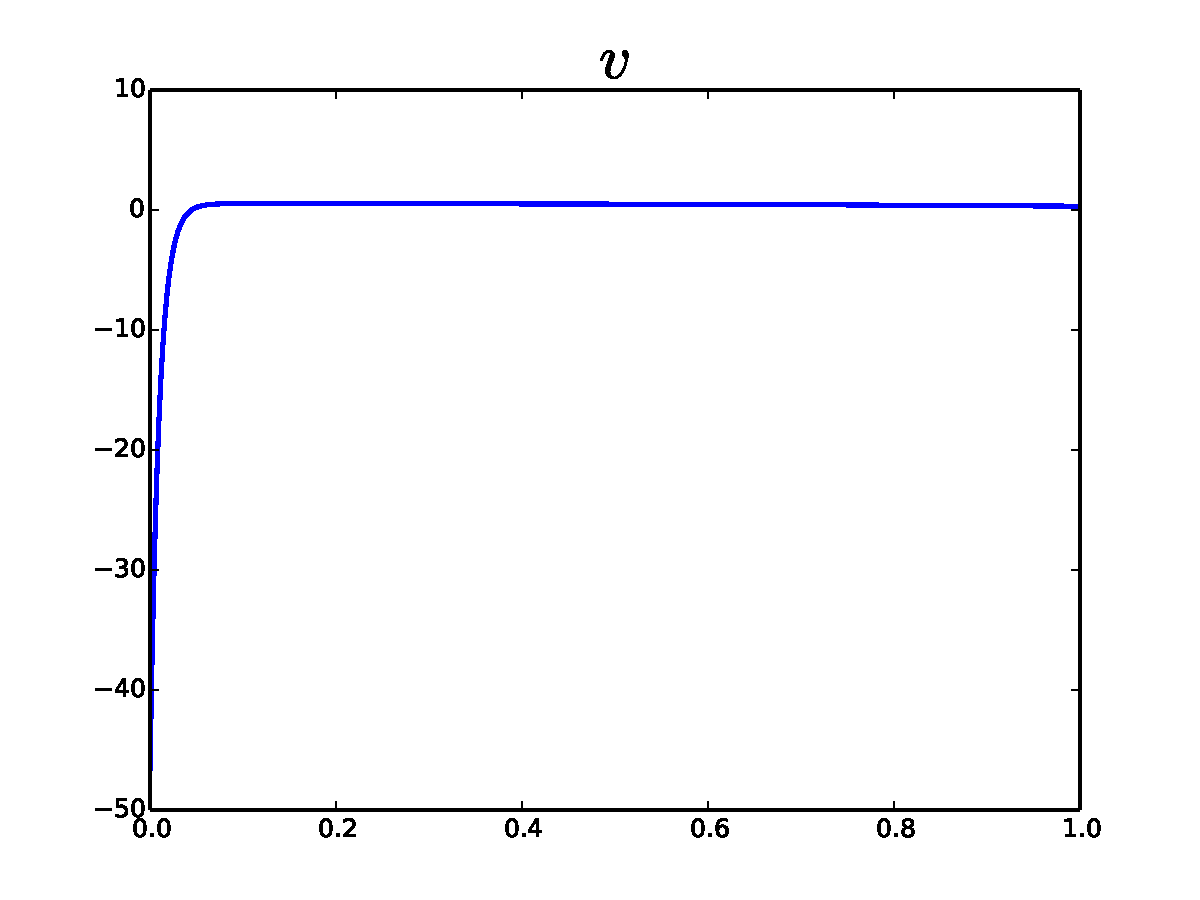
\includegraphics[width=\textwidth]{OptimalTestFunctions/Graph_v}\\
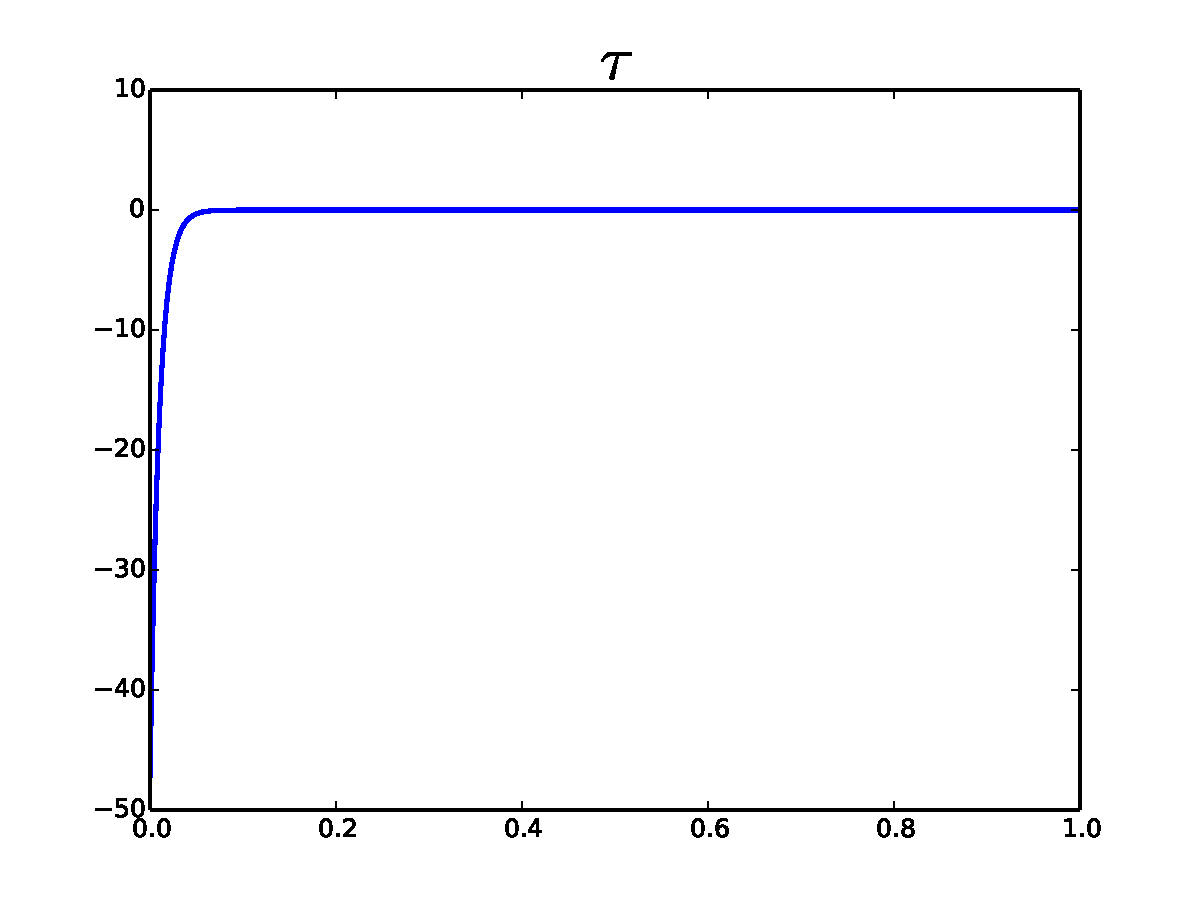
\includegraphics[width=\textwidth]{OptimalTestFunctions/Graph_tau}\\
\caption{Ideal}
\label{fig:idealGraph}
\end{subfigure}
\begin{subfigure}[t]{0.4\textwidth}
\centering
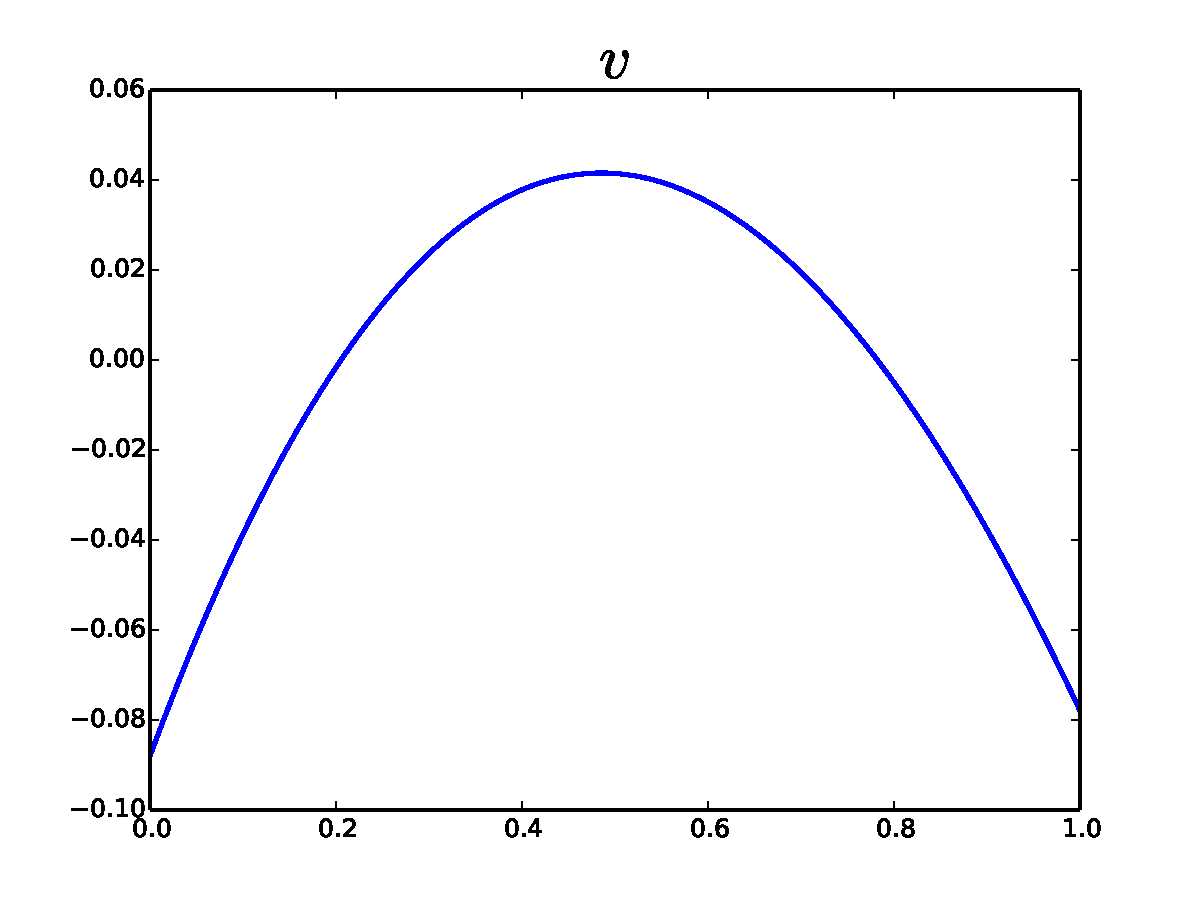
\includegraphics[width=\textwidth]{OptimalTestFunctions/GraphApprox3_v}\\
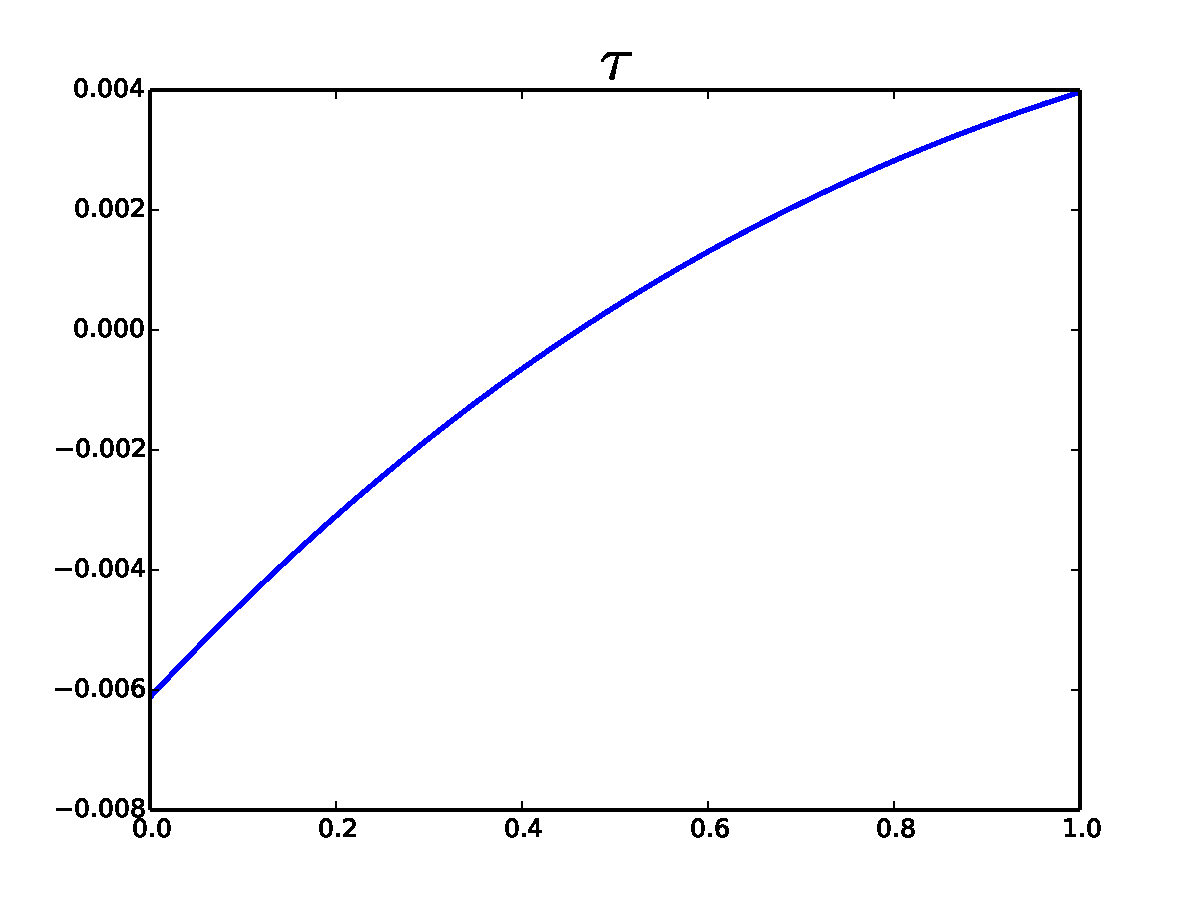
\includegraphics[width=\textwidth]{OptimalTestFunctions/GraphApprox3_tau}\\
\caption{Approximated}
\label{fig:approxGraph}
\end{subfigure}
\caption{Graph norm optimal test functions for $u=x-\frac{1}{2}$}
\label{fig:optimalGraph}
\end{figure}

\begin{figure}[ht]
\centering
\begin{subfigure}[t]{0.4\textwidth}
\centering
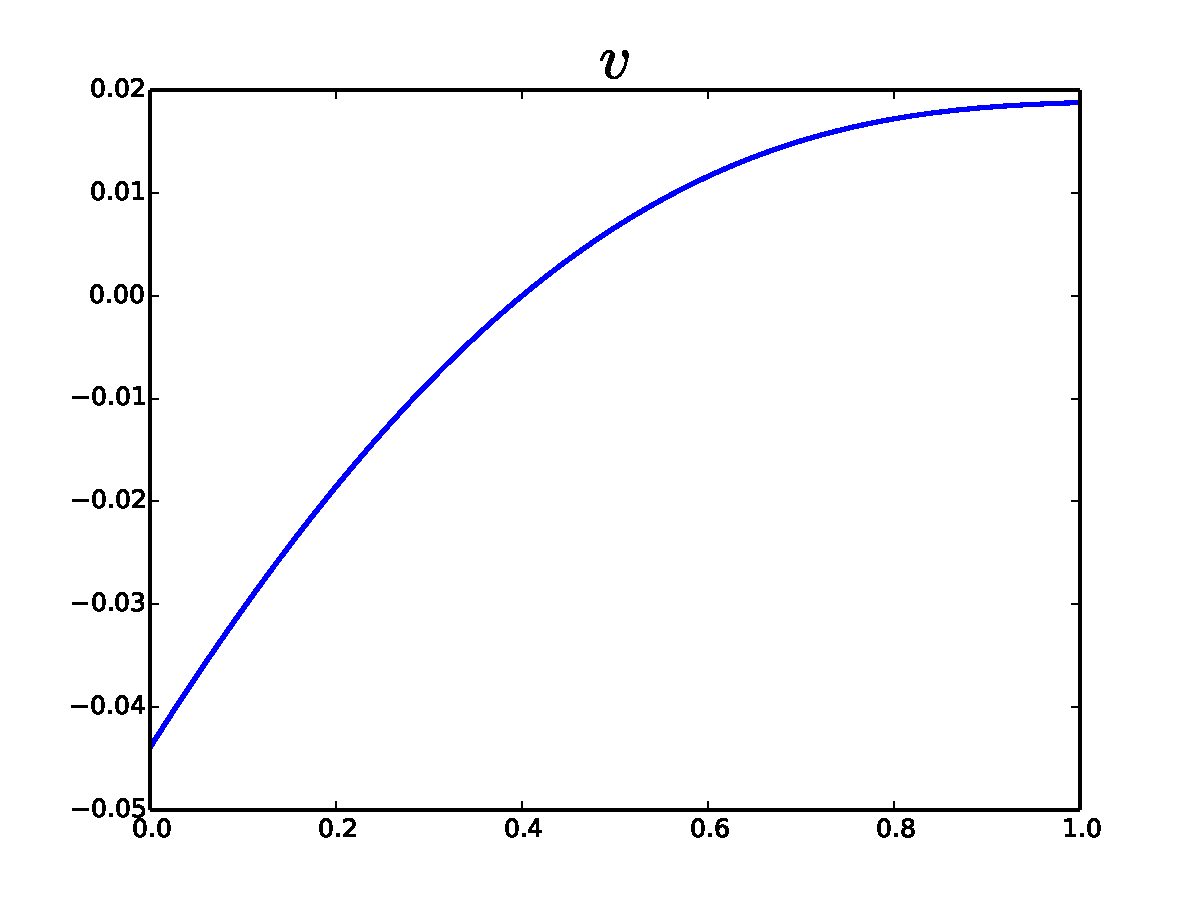
\includegraphics[width=\textwidth]{OptimalTestFunctions/Robust_v}\\
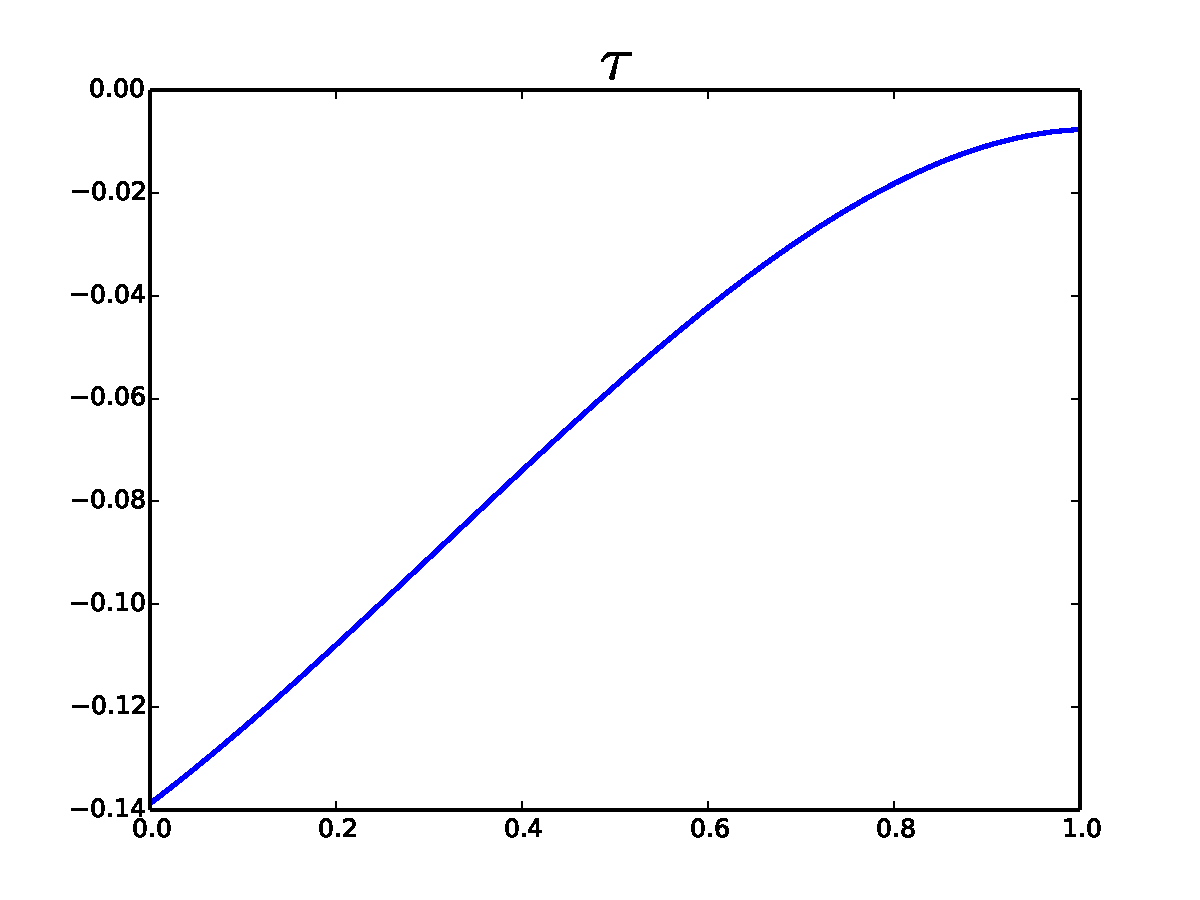
\includegraphics[width=\textwidth]{OptimalTestFunctions/Robust_tau}\\
\caption{Ideal}
\label{fig:idealRobust}
\end{subfigure}
\begin{subfigure}[t]{0.4\textwidth}
\centering
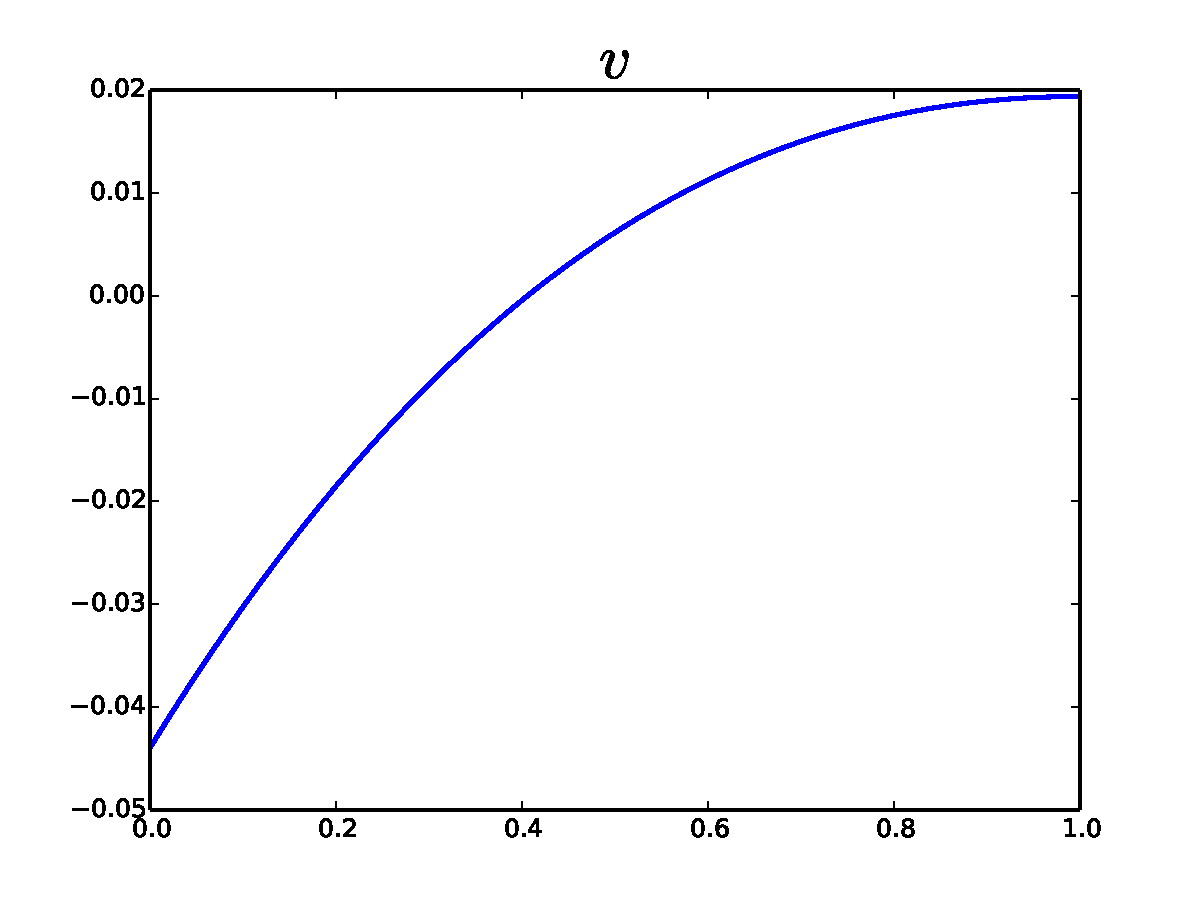
\includegraphics[width=\textwidth]{OptimalTestFunctions/RobustApprox3_v}\\
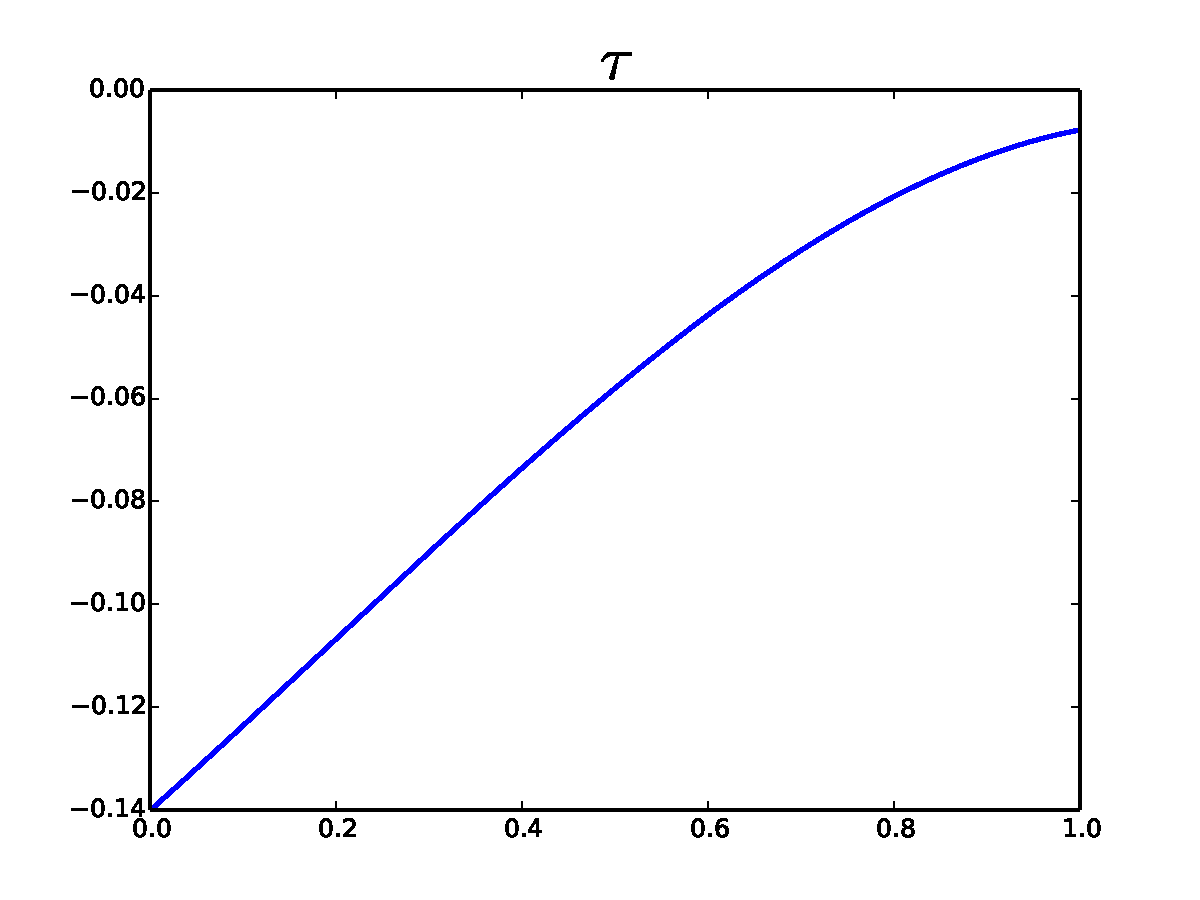
\includegraphics[width=\textwidth]{OptimalTestFunctions/RobustApprox3_tau}\\
\caption{Approximated}
\label{fig:approxRobust}
\end{subfigure}
\caption{Coupled robust norm optimal test functions for $u=x-\frac{1}{2}$}
\label{fig:optimalRobust}
\end{figure}

Mathematically, the graph norm satisfies the necessary condition to be a robust norm, but the ideal optimal test functions contain strong boundary
layers which can not be realistically approximated with the provided enriched space.
If the approximated optimal test functions can not come sufficiently close to the ideal, then the whole DPG theory falls apart.
See \cite{PracticalDPG} for more discussion.
This provides an additional condition on a test norm before we can truly call it robust: the ideal test functions must be adequately representable within 
the provided enriched space.
This ultimately comes down to an analysis of the relative magnitudes of individual terms within the test norm, usually attempting to bound reactive or convective terms by diffusive terms.
The coupled robust norm satisfies \ref{eq:necessaryCondition} and also produces relatively smooth optimal test functions that can be sufficiently approximated
with a cubic polynomial space.

\section{A Robust Norm for Transient Convection-Diffusion}

Consider transient convection-diffusion with homogeneous boundary conditions
\begin{align*}
\frac{1}{\epsilon}\bfsigma-\Grad u &=0\\
\pd{u}{t} + \bfbeta\cdot\Grad u - \Div\bfsigma &= f\\
\beta_n u-\epsilon\pd{u}{n} &= 0 \text{ on } \Gamma_-\\
u &= 0 \text{ on } \Gamma_+\\
u &= u_0 \text{ on } \Gamma_0,
\end{align*}
where $\Div\bfbeta=0$ and $\norm{\Grad\bfbeta}_{L^\infty}\le C_{\bfbeta}$.
Let $\tilde\bfbeta:=\vecttwo{\bfbeta}{1}$, then we can rewrite this as
\begin{align*}
\frac{1}{\epsilon}\bfsigma-\Grad u &=0\\
\tilde\bfbeta\cdot\Gradxt u - \Div\bfsigma &= f\\
% \Divxt\vecttwo{\bfbeta u-\bfsigma}{u}&=f\\
\beta_n u-\epsilon\pd{u}{n} &= 0 \text{ on } \Gamma_-\\
u &= 0 \text{ on } \Gamma_+\\
u &= u_0 \text{ on } \Gamma_0.
\end{align*}
We decompose the adjoint into three parts:
a discontinuous part
\textcolor{red}{(Dr. Demkowicz, what kind of argument do we want to use to avoid dealing with this part? I assume it's something to do with breaking test functions.)}
\begin{align*}
\frac{1}{\epsilon}\bftau_0+\Grad v_0 &=0\\
-\tilde\bfbeta\cdot\Gradxt v_0 + \Div\bftau_0 &= 0\\
\bftau_0\cdot\bfn_x &= \bftau\cdot\bfn_x \text{ on } \Gamma_-\cup\Gamma_0\\
v_0 &= v \text{ on } \Gamma_+\\
v_0 &= v \text{ on } \Gamma_T\\
\jump{v_0}&=\jump{v} \text{ on } \Gamma_h^0\\
\jump{\bftau_0\cdot\bfn_x}&=\jump{\bftau_0\cdot\bfn_x} \text{ on } \Gamma_{hx}^0\,,
\end{align*}
a continuous part with forcing term $g$
\begin{align*}
\frac{1}{\epsilon}\bftau_1+\Grad v_1 &=0\\
-\tilde\bfbeta\cdot\Gradxt v_1 + \Div\bftau_1 &= g\\
\bftau_1\cdot\bfn_x &= 0 \text{ on } \Gamma_-\\
v_1 &= 0 \text{ on } \Gamma_+\\
v_1 &= 0 \text{ on } \Gamma_T\,,
\end{align*}
and a continuous part with forcing $\bff$
\begin{align*}
\frac{1}{\epsilon}\bftau_2+\Grad v_2 &=\bff\\
-\tilde\bfbeta\cdot\Gradxt v_2 + \Div\bftau_2 &= 0\\
\bftau_2\cdot\bfn_x &= 0 \text{ on } \Gamma_-\\
v_2 &= 0 \text{ on } \Gamma_+\\
v_2 &= 0 \text{ on } \Gamma_T\,.
\end{align*}
(The boundary conditions can be derived by taking the ultra-weak formulation and choosing boundary conditions such that the temporal flux and spatial flux terms $\LRa{\uh, \jump{\tau_n}}_{\Gamma_{out}}$ and $\LRa{\hat t_n,\jump{v}}_{\Gamma_{in}}$ are zero.)

We can then derive that the test norm
\begin{align}
\label{eq:robustnorm}
\norm{\LRp{v,\bftau}}_{V,K}^2 &\coloneqq
\frac{1}{\epsilon}\norm{\bftau}_K^2
+ \norm{\Div \bftau - \tilde\bfbeta\cdot\Gradxt v}_K^2 \nonumber\\
&+\norm{\bfbeta\cdot \Grad v}_K^2
+ \epsilon\norm{\Grad v}_K^2
+ \norm{v}^2_K\,,
\end{align}
provides the necessary bound $\norm{v^*}_V \lesssim \norm{u}_{\LQ}$.

In the following lemmas we establish the following bounds:
\begin{itemize}
\item Bound on $\norm{\LRp{v_0,\bftau_0}}_V$. \textcolor{red}{What do we do for this?}
\item Bound on $\norm{\LRp{v_1,\bftau_1}}_V$. 
Lemma~\ref{lem:convective} gives $\norm{\tilde\bfbeta\cdot\Gradxt v_1}\leq\norm{g}$.
Since $\Div\bftau_1=g+\tilde\bfbeta\cdot\Gradxt v_1$, 
\[
\norm{\Div\bftau_1}\leq\norm{g}+\norm{\tilde\bfbeta\cdot\Gradxt v_1}\leq 2\norm{g}.
\]
Or, the fact that $\Div\bftau-\tilde\bfbeta\cdot\Gradxt v_1=g$ clearly gives
\[
\norm{\Div \bftau - \tilde\bfbeta\cdot\Gradxt v_1}=\norm{g}.
\]
Also, clearly
\[
\norm{\bfbeta\cdot\Grad v_1}\leq\norm{\tilde\bfbeta\cdot\Gradxt v_1}\leq\norm{g}.
\]
Lemma~\ref{lem:l2} gives $\norm{v_1}^2+\epsilon\norm{\Grad v_1}^2\leq\norm{g}^2$.
Since $\epsilon^{1/2}\Grad v_1=-\epsilon^{-1/2}\bftau_1$,
\[
\frac{1}{\epsilon}\norm{\bftau_1}^2\leq\norm{g}^2.
\]
Thus, all $(v_1,\bftau_1)$ terms in \eqref{eq:robustnorm} are accounted for.
\item Bound on $\norm{\LRp{v_2,\bftau_2}}_V$. 
The fact that $\Div\bftau-\tilde\bfbeta\cdot\Gradxt v=0$ clearly gives
\[
\norm{\Div \bftau - \tilde\bfbeta\cdot\Gradxt v_2}=0\leq\norm{\bff}.
\]
Lemma~\ref{lem:l2} gives $\norm{v_2}^2+\epsilon\norm{\Grad v_2}^2\leq\epsilon\norm{\bff}^2$.
Since $\epsilon^{1/2}\Grad v_2=\bff-\epsilon^{-1/2}\bftau_2$,
\[
\frac{1}{\epsilon}\norm{\bftau_2}^2\leq(1+\epsilon)\norm{\bff}^2.
\]
Finally,
\[
\norm{\bfbeta\cdot\Grad v_2}\leq\norm{\bfbeta}_\infty\norm{\Grad v_2}\leq\norm{\bfbeta}_\infty\norm{\bff}.
\]
Thus, all $(v_2,\bftau_2)$ terms in \eqref{eq:robustnorm} are accounted for.
\end{itemize}

Our goal is to analyze the stability properties of the adjoint equations by deriving bounds of the form
$\norm{(v_1,\bftau_1)}_V\leq\norm{g}_\LQ$ and $\norm{(v_2,\bftau_2)}_V\leq\norm{f}_\LQ$.

% \textcolor{red}{Insert conditions on $\bfbeta$}
\begin{lemma}
\label{lem:convective}
% For the above conditions on $\bfbeta$,
% If 
% \[
% \norm{\Grad\bfbeta-\frac{1}{2}\Div\bfbeta\bfI}_L^{\infty}\le C_{\bfbeta}
% \]
% then
We can bound
\[
\norm{\tilde\bfbeta\cdot\Gradxt v_1}\leq \norm{g}.
\]
\end{lemma}
\begin{proof}
Multiply $-\tilde\bfbeta\cdot\Gradxt v=g-\Div\bftau$ by $-\tilde\bfbeta\cdot\Gradxt v$ and integrate over $Q$ to get
\begin{equation}
\label{eq:adj1}
\norm{\tilde\bfbeta\cdot\Gradxt v}^2=-\int_Q g\tilde\bfbeta\cdot\Gradxt v+\int_Q\tilde\bfbeta\cdot\Gradxt v\Div\bftau\,.
\end{equation}
Note that
\begin{align*}
\frac{1}{\epsilon}\int_Q\tilde\bfbeta\cdot\Gradxt v\Div\bftau&=-\int_Q\tilde\bfbeta\cdot\Gradxt v\Div\Grad v \\
%
&=-\int_{\Gamma_x}\tilde\bfbeta\cdot\Gradxt v\Grad v\cdot\bfn_x
+\int_Q\Grad(\tilde\bfbeta\cdot\Gradxt v)\cdot\Grad v \\
%
&=-\int_{\Gamma_x}\tilde\bfbeta\cdot\Gradxt v\Grad v\cdot\bfn_x
+\int_Q(\Grad\tilde\bfbeta\cdot\Gradxt v)\cdot\Grad v\\
&\quad+\int_Q\tilde\bfbeta\cdot\Grad\Gradxt v\cdot\Grad v\\
%
&=-\int_{\Gamma_x}\tilde\bfbeta\cdot\Gradxt v\Grad v\cdot\bfn_x
+\int_Q(\Grad\bfbeta\cdot\Grad v)\cdot\Grad v\\
&\quad+\frac{1}{2}\int_Q\tilde\bfbeta\cdot\Gradxt(\Grad v\cdot\Grad v)\\
%
&=-\int_{\Gamma_x}\tilde\bfbeta\cdot\Gradxt v\Grad v\cdot\bfn_x
+\int_Q(\Grad\bfbeta\cdot\Grad v)\cdot\Grad v\\
&\quad+\frac{1}{2}\int_\Gamma\tilde\bfbeta\cdot\bfn(\Grad v\cdot\Grad v)
-\frac{1}{2}\int_Q\Divxt\tilde\bfbeta(\Grad v\cdot\Grad v)\\
%
&=-\int_{\Gamma_x}\tilde\bfbeta\cdot\Gradxt v\Grad v\cdot\bfn_x
+\int_Q(\Grad\bfbeta\cdot\Grad v)\cdot\Grad v\\
&\quad+\frac{1}{2}\int_\Gamma\tilde\bfbeta\cdot\bfn(\Grad v\cdot\Grad v)
-\frac{1}{2}\int_Q\Div\bfbeta(\Grad v\cdot\Grad v)\\
%
&=-\int_{\Gamma_x}\tilde\bfbeta\cdot\Gradxt v\Grad v\cdot\bfn_x
+\frac{1}{2}\int_\Gamma\tilde\bfbeta\cdot\bfn(\Grad v\cdot\Grad v)\\
&\quad+\int_Q\Grad v(\Grad\bfbeta-\frac{1}{2}\Div\bfbeta\bfI)\Grad v\\
\end{align*}
Plugging this into \eqref{eq:adj1}, we get
\begin{align*}
\norm{\tilde\bfbeta\cdot\Gradxt v}^2
&=-\int_Q g\tilde\bfbeta\cdot\Gradxt v
+\epsilon\int_Q\Grad v(\Grad\bfbeta-\frac{1}{2}\Div\bfbeta\bfI)\Grad v\\
&\quad-\epsilon\int_{\Gamma_x}\tilde\bfbeta\cdot\Gradxt v\Grad v\cdot\bfn_x
+\frac{\epsilon}{2}\int_\Gamma\tilde\bfbeta\cdot\bfn(\Grad v\cdot\Grad v)\\
%
&=-\int_Q g\tilde\bfbeta\cdot\Gradxt v
+\epsilon\int_Q\Grad v(\Grad\bfbeta-\frac{1}{2}\Div\bfbeta\bfI)\Grad v\\
&\quad
-\epsilon\int_{\Gamma_-}\tilde\bfbeta\cdot\Gradxt v\underbrace{\Grad v\cdot\bfn_x}_{=0}
-\epsilon\int_{\Gamma_+}\LRp{\underbrace{\pd{v}{t}}_{=0}+\bfbeta\cdot\Grad v}\Grad v\cdot\bfn_x\\
&\quad
+\frac{\epsilon}{2}\int_{\Gamma_-}\underbrace{\bfbeta\cdot\bfn_x}_{<0}(\Grad v\cdot\Grad v)
+\frac{\epsilon}{2}\int_{\Gamma_+}\bfbeta\cdot\bfn_x(\Grad v\cdot\Grad v)\\
&\quad
+\frac{\epsilon}{2}\int_{\Gamma_0}\underbrace{n_t}_{<0}(\Grad v\cdot\Grad v)
+\frac{\epsilon}{2}\int_{\Gamma_T}n_t\underbrace{(\Grad v\cdot\Grad v)}_{=0}\\
%
&\leq-\int_Q g\tilde\bfbeta\cdot\Gradxt v
+\epsilon\int_Q\Grad v(\Grad\bfbeta-\frac{1}{2}\Div\bfbeta\bfI)\Grad v\\
&\quad
+\epsilon\int_{\Gamma_+}\LRp{-\pd{v}{\bfn_x}\bfbeta
+\frac{1}{2}\bfbeta\cdot\bfn_x\Grad v}\cdot\Grad v\\
%
&=-\int_Q g\tilde\bfbeta\cdot\Gradxt v
+\epsilon\int_Q\Grad v(\Grad\bfbeta-\frac{1}{2}\Div\bfbeta\bfI)\Grad v\\
&\quad
+\epsilon\int_{\Gamma_+}\LRp{-\pd{v}{\bfn_x}\bfbeta
+\frac{1}{2}\bfbeta\cdot\bfn_x\pd{v}{\bfn_x}\bfn_x}\cdot\pd{v}{\bfn_x}\bfn_x\\
%
&=-\int_Q g\tilde\bfbeta\cdot\Gradxt v
+\epsilon\int_Q\Grad v(\Grad\bfbeta-\frac{1}{2}\Div\bfbeta\bfI)\Grad v\\
&\quad
\underbrace{-\frac{\epsilon}{2}\int_{\Gamma_+}\LRp{\pd{v}{\bfn_x}}^2\bfbeta\cdot\bfn_x}_{<0}\\
%
&\leq-\int_Q g\tilde\bfbeta\cdot\Gradxt v
+\epsilon\int_Q\Grad v(\Grad\bfbeta-\frac{1}{2}\Div\bfbeta\bfI)\Grad v\\
%
&\leq\frac{\norm{g}^2}{2}+\frac{\norm{\tilde\bfbeta\cdot\Gradxt v}^2}{2}
+\epsilon\int_Q\Grad v(\Grad\bfbeta-\frac{1}{2}\Div\bfbeta\bfI)\Grad v\\
%
&\leq\frac{\norm{g}^2}{2}+\frac{\norm{\tilde\bfbeta\cdot\Gradxt v}^2}{2}
+\epsilon C_{\bfbeta}\norm{\Grad v}^2
\end{align*}
\textcolor{red}{
Seems to additionally require that $\epsilon C_{\bfbeta}\norm{\Grad v}^2\le\norm{\tilde\bfbeta\cdot\Gradxt v}^2$.
}
\end{proof}

\begin{lemma}
\label{lem:l2}
For the duration of this lemma, let $v:=v_1+v_2$.
Then, for the above conditions on $\bfbeta$,
\[
\norm{v}^2+\epsilon\norm{\Grad v}^2\leq\norm{g}^2+\epsilon\norm{\bff}^2\,.
\]
\end{lemma}
\begin{proof}
Define $w=e^{t}v$ and note that $\pd{w}{t}=\LRp{\pd{v}{t}+v}e^{t}$ while
all spatial derivatives go through.
%  $\Grad w=\cancelto{0}{\Grad e^{t}} v+e^{t}\Grad v$ and
% $\Div(\bfbeta w)=\Div(\bfbeta)e^{t} v+\bfbeta\cdot e^{t}\Grad v$ and $\Delta w=e^{t}\Delta v$. 
% Also, $\Gradxt w=\pd{e^{t} v}{t}+\Grad{e^{t} v}=e^{t}(\Gradxt v-v)$.
% Plugging this into the adjoint equation, we get
Multiplying the adjoint by $w$ and integrating over $Q$ gives
% \begin{equation*}
% -\tilde\bfbeta\cdot\Gradxt(w)-\epsilon\Delta w=g-\epsilon\Div\bff
% \end{equation*}
% or 
% \begin{equation*}
% \tilde\bfbeta\cdot\Gradxt(v)-v+\epsilon\Delta v=e^{t}(-g+\epsilon\Div\bff)
% \end{equation*}
% Multiply by $-v$ and integrate to get
\begin{align*}
-\int_Q\tilde\bfbeta\cdot\Gradxt vw-\epsilon\Delta vw=\int_Qgw-\epsilon\int_Q\Div\bff w
\end{align*}
or
\begin{align*}
-\int_Qe^{t}v\tilde\bfbeta\cdot\Gradxt v-\epsilon\int_Q e^{t}v\Delta v=\int_Qe^{t}gv-\epsilon\int_Qe^{t}v\Div\bff
\end{align*}
Integrating by parts:
\begin{align*}
\int_Q\Divxt\LRp{e^{t}\tilde\bfbeta v}v&
-\int_\Gamma e^{t}\tilde\bfbeta\cdot\bfn v^2
+\epsilon\int_Qe^{t}\Grad v\cdot\Grad v
-\epsilon\int_{\Gamma_x}e^{t}v\cdot\Grad v\cdot\bfn_x
\\
&=
\int_Qe^{t}gv
+\epsilon\int_Qe^{t}\Grad v\cdot\bff
-\epsilon\int_{\Gamma_x}e^{t}v\bff\cdot\bfn_x
\end{align*}
Note that $\Divxt{e^{t}v\tilde\bfbeta}=e^{t}(\tilde\bfbeta\cdot\Gradxt v+v)$ if $\Div\bfbeta=0$.
% Dividing both sides by $e^{t}$ and moving some terms to the right hand side, we get
Moving some terms to the right hand side, we get
\begin{align*}
\int_Q e^{t}v^2
&+\int_Q\epsilon e^{t}\Grad v\cdot\Grad v
\\
&=
\int_Qe^{t}gv
+\epsilon\int_Qe^{t}\Grad v\cdot\bff
-\epsilon\int_{\Gamma_x}e^{t}v\bff\cdot\bfn_x\\
&\quad-\int_Qe^{t}\tilde\bfbeta\cdot\Gradxt vv
\quad+\int_\Gamma e^{t}\tilde\bfbeta\cdot\bfn v^2
\quad+\epsilon\int_{\Gamma_x}e^{t}v\cdot\Grad v\cdot\bfn_x
\end{align*}
Note that $1\leq\norm{e^t}_\infty=e^T$, 
then
\begin{align*}
\norm{v}^2
&+\epsilon\norm{\Grad v}^2
\\
&\leq
e^T\left(
\int_Qgv
+\epsilon\int_Q\Grad v\cdot\bff
-\epsilon\int_{\Gamma_-}v\underbrace{\bff\cdot\bfn_x}_{=\cancelto{0}{\tau_n}+\pd{v}{\bfn_x}}
-\epsilon\int_{\Gamma_+}\underbrace{v}_{=0}\bff\cdot\bfn_x
\right.\\
&\left.
\quad-\int_Q\tilde\bfbeta\cdot\Gradxt vv
\quad+\int_\Gamma \tilde\bfbeta\cdot\bfn v^2
\quad+\epsilon\int_{\Gamma_-}v\cdot\Grad v\cdot\bfn_x
\quad+\epsilon\int_{\Gamma_+}\underbrace{v}_{=0}\pd{v}{\bfn_x}
\right)
\\
&=
e^T\left(
\int_Qgv
+\epsilon\int_Q\Grad v\cdot\bff
\cancel{
-\epsilon\int_{\Gamma_-}v\pd{v}{\bfn_x}
\quad+\epsilon\int_{\Gamma_x}v\pd{v}{\bfn_x}
}
\right.\\
&\left.
\quad-\frac{1}{2}\int_Q\tilde\bfbeta\cdot\Gradxt v^2
\quad+\int_\Gamma \tilde\bfbeta\cdot\bfn v^2
\right)
\\
&=
e^T\left(
\int_Qgv
+\epsilon\int_Q\Grad v\cdot\bff
\right)\\
&\left.
\quad+\frac{1}{2}\int_Q\cancelto{0}{\Divxt\tilde\bfbeta} v^2
\quad-\frac{1}{2}\int_\Gamma\tilde\bfbeta\cdot\bfn v^2
\quad+\int_\Gamma \tilde\bfbeta\cdot\bfn v^2
\right)
\\
&=
e^T\left(
\int_Qgv
+\epsilon\int_Q\Grad v\cdot\bff
\right.\\
&\left.
\quad+\frac{1}{2}\LRp{\int_{\Gamma_0} \underbrace{-v^2}_{\leq 0}
\quad+\int_{\Gamma_T} \cancelto{0}{v^2}
\quad+\int_{\Gamma_-} \underbrace{\bfbeta\cdot\bfn_x v^2}_{\leq 0}
\quad+\int_{\Gamma_+} \bfbeta\cdot\bfn_x \cancelto{0}{v^2}
}
\right)
\\
&\leq
e^T\left(
\int_Qgv
+\epsilon\int_Q\Grad v\cdot\bff
\right)
\\
&\leq
e^T\left(
\frac{\norm{g}^2}{2}
+\epsilon\frac{\norm{\bff}^2}{2}
+\frac{\norm{v}^2}{2}
+\epsilon\frac{\norm{\Grad v}^2}{2}
\right)
\end{align*}
\end{proof}

\section{Numerical Tests}

\begin{figure}[ht]
\centering
\begin{subfigure}[t]{0.4\textwidth}
\centering
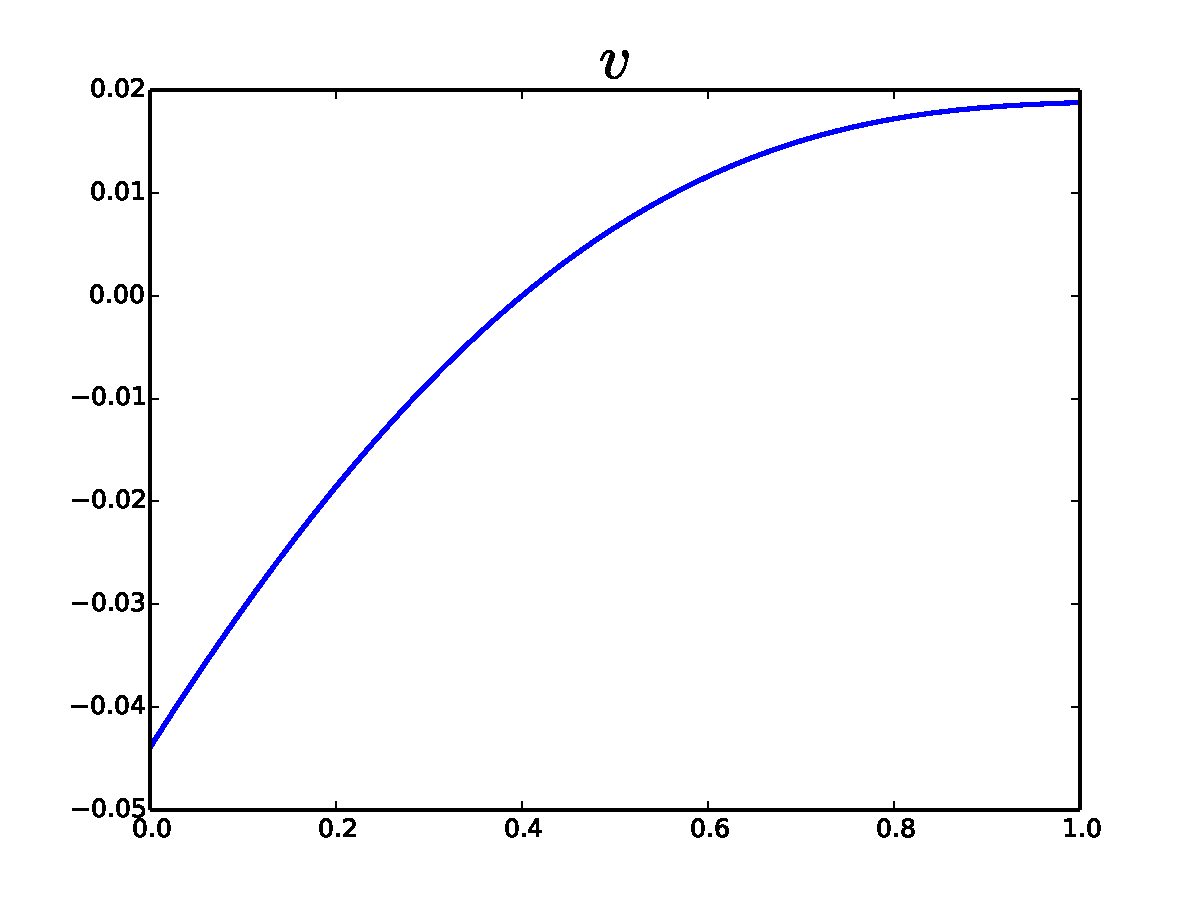
\includegraphics[width=\textwidth]{OptimalTestFunctions/Robust_v}\\
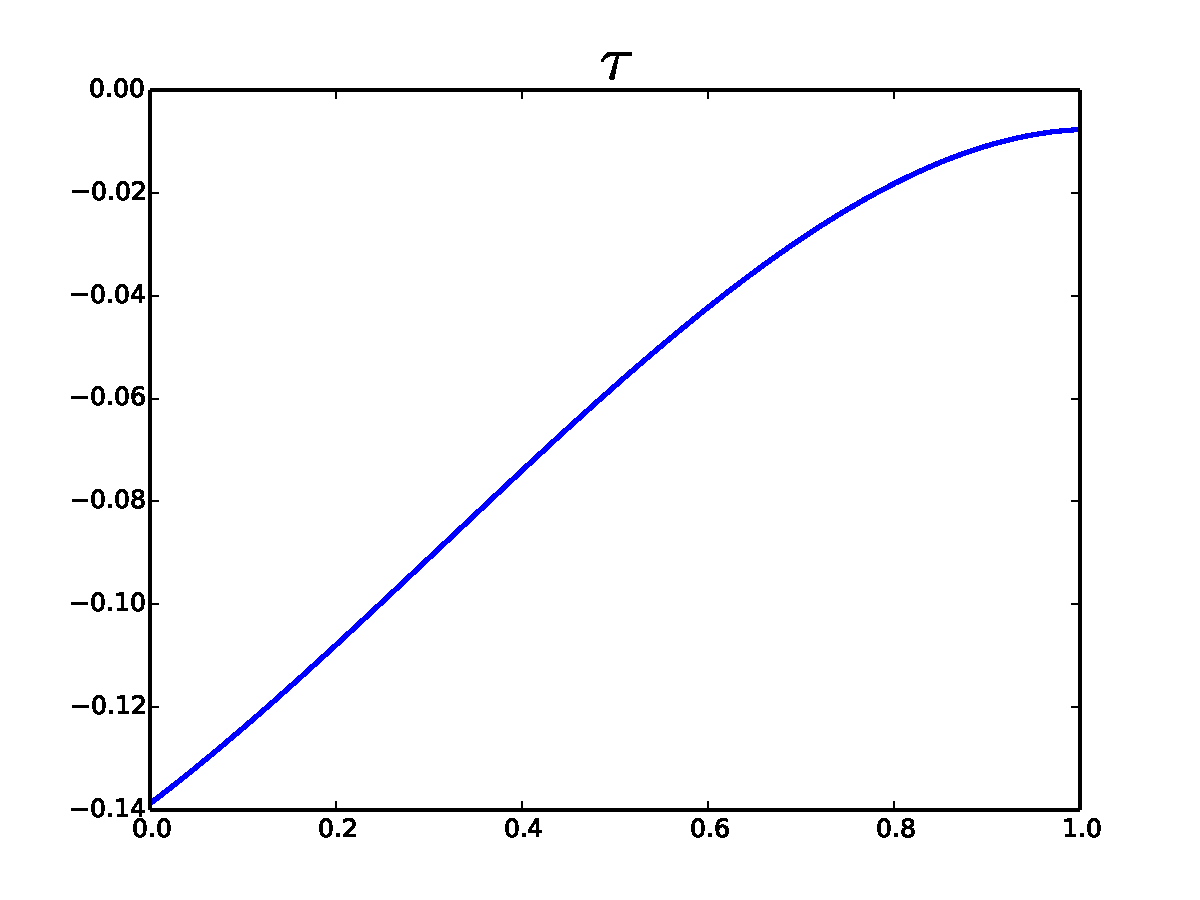
\includegraphics[width=\textwidth]{OptimalTestFunctions/Robust_tau}\\
\caption{Ideal}
\label{fig:idealRobust}
\end{subfigure}
\begin{subfigure}[t]{0.4\textwidth}
\centering
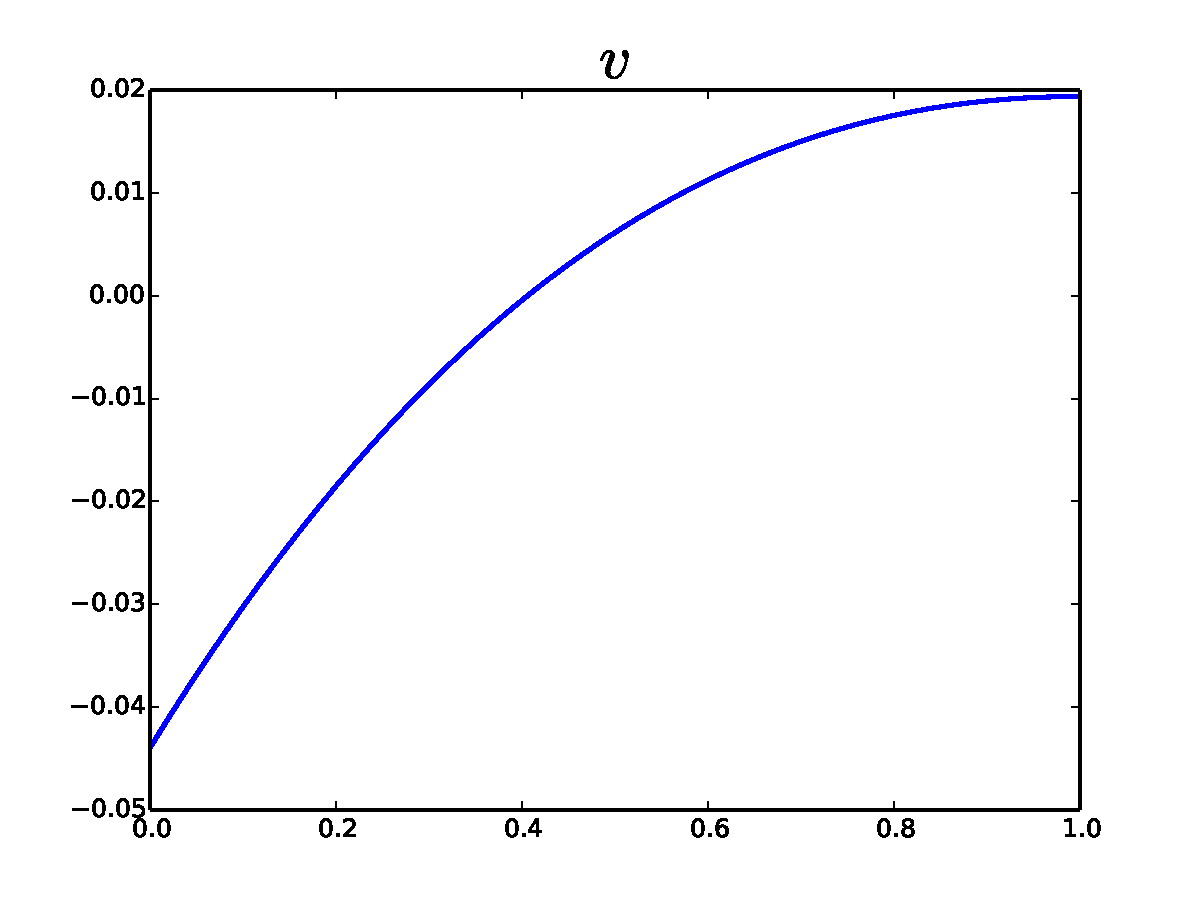
\includegraphics[width=\textwidth]{OptimalTestFunctions/RobustApprox3_v}\\
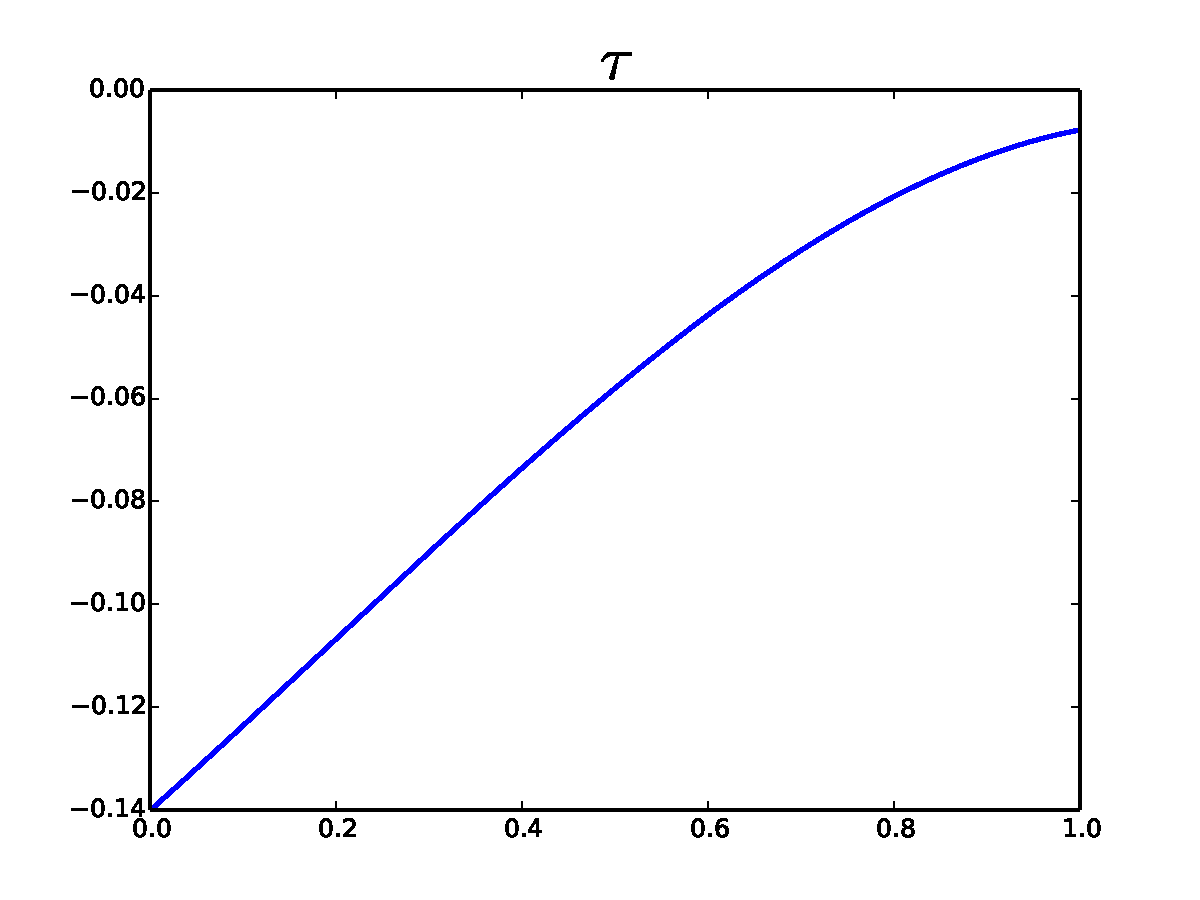
\includegraphics[width=\textwidth]{OptimalTestFunctions/RobustApprox3_tau}\\
\caption{Approximated}
\label{fig:approxRobust}
\end{subfigure}
\caption{Coupled robust norm optimal test functions for $u=x-\frac{1}{2}$}
\label{fig:optimalRobust}
\end{figure}

\bibliographystyle{elsarticle-num} 
\bibliography{../Papers}

\end{document}